\documentclass[14pt]{beamer}

\mode<presentation>
{
  \usetheme{default}
  % or ...

  \setbeamercovered{transparent}
  % or whatever (possibly just delete it)
}


\usepackage[english]{babel}
\usepackage[utf8]{inputenc}
\usepackage{listings}

% \usepackage{times}
% \usepackage[T1]{fontenc}
% Or whatever. Note that the encoding and the font should match. If T1
% does not look nice, try deleting the line with the fontenc.


\title{How the PyPy JIT works}

\author{Benjamin Peterson \\ benjamin@python.org}
% - Use the \inst{?} command only if the authors have different
%   affiliation.

\date{PyCon 2012}


% If you have a file called "university-logo-filename.xxx", where xxx
% is a graphic format that can be processed by latex or pdflatex,
% resp., then you can add a logo as follows:

% \pgfdeclareimage[height=0.5cm]{university-logo}{university-logo-filename}
% \logo{\pgfuseimage{university-logo}}


% If you wish to uncover everything in a step-wise fashion, uncomment
% the following command: 

%\beamerdefaultoverlayspecification{<+->}

\lstset{basicstyle=\scriptsize\ttfamily}


\begin{document}

\begin{frame}
  \titlepage
\end{frame}

% Since this a solution template for a generic talk, very little can
% be said about how it should be structured. However, the talk length
% of between 15min and 45min and the theme suggest that you stick to
% the following rules:  

% - Exactly two or three sections (other than the summary).
% - At *most* three subsections per section.
% - Talk about 30s to 2min per frame. So there should be between about
%   15 and 30 frames, all told.

\begin{frame}
  % - A title should summarize the slide in an understandable fashion
  %   for anyone how does not follow everything on the slide itself.

  ``If the implementation is hard to explain, it's a bad idea.''
  \vskip0pt plus.5fill
  \uncover<2->{Except PyPy!}
\end{frame}

\begin{frame}{Design Principles}
\begin{itemize}
\item interpreter agnostic
\item but allow language implementation to help JIT
\item compile hot code: loops or functions
\item use runtime information to remove dynamic overhead
\item optimize common and idiomatic code
\end{itemize}
\end{frame}

\begin{frame}{Overview}
\begin{itemize}
\item translation
\item runtime
\begin{itemize}
\item tracing
\item optimization
\item assembly generation
\end{itemize}
\end{itemize}
\end{frame}

\begin{frame}[fragile]{Adding JIT to an interpreter}
\begin{itemize}
\item JIT args
\begin{itemize}
\item ``greens'' = constants
\item ``reds'' = variables
\end{itemize}
\item hints
\begin{itemize}
\item \verb+can_enter_jit+
\item \verb+jit_merge_point+
\end{itemize}
\end{itemize}
\end{frame}

\begin{frame}[fragile]{JIT on the Python interpreter}
\begin{itemize}
\item greens: code object and instruction pointer
\item reds: frame object and execution context
\end{itemize}
\begin{lstlisting}[language=Python]
while True:
    jit_merge_point()
    next_instr = self.handle_bytecode(code, next_instr)
\end{lstlisting}
\begin{lstlisting}[language=Python]
def JUMP_ABSOLUTE(jump_to):
    can_enter_jit()
    return jump_to
\end{lstlisting}
\end{frame}

\begin{frame}{Generating the JIT}
\begin{itemize}
\item RPython interpreter is in low-level flowgraphs
\item low-level flowgraphs converted to jitcodes
\item interpreter decides what functions to ``look into''
\item jitcodes stored in binary
\end{itemize}
\end{frame}

\begin{frame}[fragile]{Main example: Primality Test}
\begin{lstlisting}[language=Python]
def is_prime(n):
    limit = int(n**.5)
    i = 2
    while i <= limit:
        if n % i == 0:
            return False
        i += 1
    return True
\end{lstlisting}
\end{frame}

\begin{frame}[fragile]{Primality Test - Bytecode}
\tiny{
\begin{verbatim}
# while i <= limit:
22 SETUP_LOOP         46 (to 71)
25 LOAD_FAST          2 (i)
28 LOAD_FAST          1 (limit)
31 COMPARE_OP         1 (<=)
34 POP_JUMP_IF_FALSE  70
# if i % 1 === 0:
37 LOAD_FAST          0 (n)
40 LOAD_FAST          2 (i)
43 BINARY_MODULO       
44 LOAD_CONST         3 (0)
47 COMPARE_OP         2 (==)
50 POP_JUMP_IF_FALSE  57
#     return False
53 LOAD_GLOBAL        1 (False)
56 RETURN_VALUE        
# i += 1
57 LOAD_FAST          2 (i)
60 LOAD_CONST         4 (1)
63 INPLACE_ADD         
64 STORE_FAST         2 (i)
67 JUMP_ABSOLUTE      25
\end{verbatim}
}
\end{frame}

\begin{frame}[fragile]{Activating the JIT}
\begin{itemize}
\item every loop has a counter incremented when \verb+can_enter_jit+ is reached
\item tracing entered when threshold reached
\item slight fudging to avoid compiling everything suddenly
\end{itemize}
\end{frame}

\begin{frame}{Tracing}
\begin{itemize}
\item metainterpreter executes saved jitcodes
\item records operations in JIT IR
\item traces through function calls, flattening loop
\item program values stored in boxes (pointers, integers, floats)
\item tracing ends when loop is closed
\end{itemize}
\end{frame}

\begin{frame}{Guards}
\begin{itemize}
\item as the jit traces, it makes assumptions based on runtime information
\item these must hold otherwise trace is invalid
\item guards protect trace from different runtime conditions
\item examples: conditional branches, overflow, exceptions, other code accessing JIT data
\end{itemize}
\end{frame}

\begin{frame}[fragile]{JIT IR example - Head of loop}
\footnotesize{
\begin{verbatim}
# arguments to loop
[p0, p1, p2, p3, i4, p5, i6, i7, p8, p9, p10, p11, p12, p13]
#25 LOAD_FAST
guard_value(i6, 3)
guard_nonnull(p10)
guard_value(i4, 0)
#28 LOAD_FAST
guard_nonnull(p9)
#31 COMPARE_OP
guard_class(p10, W_IntObject)
guard_class(p9, W_IntObject)
i18 = getfield_gc_pure(p10, <W_IntObject.inst_intval>)
i19 = getfield_gc_pure(p9, <W_IntObject.inst_intval>)
i20 = int_le(i18, i19)
guard_true(i20)
#34 POP_JUMP_IF_FALSE
\end{verbatim}
}
\end{frame}

\begin{frame}[fragile]{JIT IR example - computing modulo}
\footnotesize{
\begin{verbatim}
#37 LOAD_FAST
guard_nonnull(p8)
#40 LOAD_FAST
#43 BINARY_MODULO
guard_class(p8, W_IntObject)
i22 = getfield_gc_pure(p8, <W_IntObject.inst_intval>)
i23 = int_is_zero(i18)
guard_false(i23)
i25 = int_eq(i22, -9223372036854775808)
guard_false(i25)
i26 = int_mod(i22, i18)
i28 = int_lt(i18, 0)
guard_false(i28)
i30 = int_rshift(i26, 63)
i31 = int_and(i18, i30)
i32 = int_add(i26, i31)
p34 = new_with_vtable(W_IntObject)
setfield_gc(p34, i32, <W_IntObject.inst_intval>)
\end{verbatim}
}
\end{frame}

\begin{frame}[fragile]{JIT IR example - check modulo}
\footnotesize{
\begin{verbatim}
#44 LOAD_CONST
guard_value(p3, ConstPtr(ptr35))
#47 COMPARE_OP')
i37 = int_eq(i32, 0)
guard_false(i37)
#50 POP_JUMP_IF_FALSE
\end{verbatim}
}
\end{frame}

\begin{frame}[fragile]{JIT IR example - finish loop}
\footnotesize{
\begin{verbatim}
#57 LOAD_FAST
#60 LOAD_FAST
#63 INPLACE_ADD
i38 = getfield_gc_pure(p10, <W_IntObject.inst_intval>)
i40 = int_add_ovf(i38, 1)
guard_no_overflow()
p42 = new_with_vtable(W_IntObject)
setfield_gc(p42, i40, <W_IntObject.inst_intval>)
#64 STORE_FAST
#67 JUMP_ABSOLUTE
\end{verbatim}
}
\end{frame}

\begin{frame}{Optimizations}
\begin{itemize}
\item limited by speed
\item classical compiler optimizations
\begin{itemize}
\item constant folding
\item strength reduction
\item integer bounds
\end{itemize}
\item remove extra gaurds
\item most important is removing indirection: virtuals and virtualizables
\end{itemize}
\end{frame}

\begin{frame}{Virtuals}
\begin{itemize}
\item if objects allocated in the loop don't escape it, we don't have to
  allocate them
\item removes boxing
\item all field access can be killed
\item in our example, removes integer allocations
\end{itemize}
\end{frame}

\begin{frame}{Virtualizables}
\begin{itemize}
\item like virtuals but allowed to escape trace
\item handled at metainterp level
\item Python interpreter: the frame object
\item possibility of escape creates bookkeeping problems
\item advantage of JIT generator approach
\end{itemize}
\end{frame}

\begin{frame}{Unrolling}
\begin{itemize}
\item need some way to compute loop invariants before reaching optimized loop
\item solution: two optimization passes
\item first iteration computes loop invariants
\item second iteration is tight loop
\end{itemize}
\end{frame}

\begin{frame}{JIT viewer}
Our fancy toy for visualizing JIT
\end{frame}

\begin{frame}{Creating assembly}
\begin{itemize}
\item surprisingly straightforward
\item linear register allocator
\item gc has to be informed of dynamic allocations
\item assembly now ready to be run
\end{itemize}
\end{frame}

\begin{frame}{Bailing from the JIT}
\begin{itemize}
\item guards fail while assembly is running
\item assembler has written a compact description of hower to recover state
\item state reconstructed
\item blackhole interpreter
\item if gaurd fails repeatedly, compile a bridge
\end{itemize}
\end{frame}

\begin{frame}[fragile]{How the Python interpreter helps the JIT}
\begin{itemize}
\item constant promotion
\item decorators: \verb+unroll_safe+, \verb+elidable+
\item data structures optimized for the JIT
\begin{itemize}
\item map dicts
\item cell dicts
\item list and dict strategies
\item specialized tuples
\end{itemize}
\end{itemize}
\end{frame}

\begin{frame}{Map dicts}
\begin{itemize}
\item shares object attributes
\item instance data stored in array
\item memory efficient as well as good for the JIT
\end{itemize}
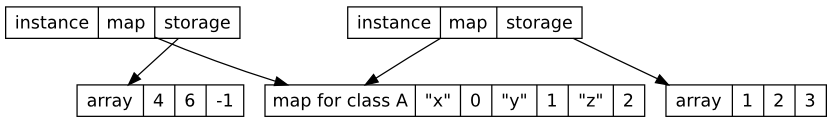
\includegraphics[scale=.45]{instancemap.png}
\end{frame}

\begin{frame}[fragile]{Thank you}
Questions?

Resources
\begin{itemize}
\item \#pypy on Freenode
\item http://morepypy.blogspot.com
\item pypy-dev@python.org
\item The Architecture of Open Source Applications, Volume 2
\end{itemize}


My email: benjamin@python.org
\end{frame}

\end{document}
